\chapter{Titrages pH-métriques et conductimétriques}\label{ch:g12:ph-conductivity-titrations}

L'étiquette d'une bouteille de vinaigre de vin indique «~6~\% d'acidité~»~:
six grammes d'acide éthanoïque pour cent grammes de vinaigre. Ni l'acide
éthanoïque ni sa base conjuguée ne sont colorés, et aucun permanganate
ne sera utile ici. Mais un \omterm{def:g9:acids-bases-ph:ph-paper}{pH-mètre} plongé dans le vinaigre, ou une
cellule qui mesure sa capacité à conduire le courant, suit goutte à
goutte la réaction avec une base, et la forme de la courbe montre
exactement où se trouve l'\omterm{def:g11:titration:equivalence}{équivalence}. Dix minutes à la paillasse, et
l'étiquette est vérifiée.

\begin{recall}
Un \omterm{def:g11:titration:titration}{titrage}, son \omterm{def:g11:titration:equivalence}{équivalence} et son \omterm{def:g11:titration:equivalence}{volume à l'équivalence}
(\cref{ch:g11:titration})~; les \omterm{def:g12:ka-and-pka:ka}{constantes d'acidité}
(\cref{ch:g12:ka-and-pka})~; la relation de Henderson et les indicateurs
colorés (\cref{ch:g12:buffers-predominance})~; les solutions ioniques
conduisent le courant électrique (\cref{ch:g9:ions}).
\end{recall}

\begin{omfigure}
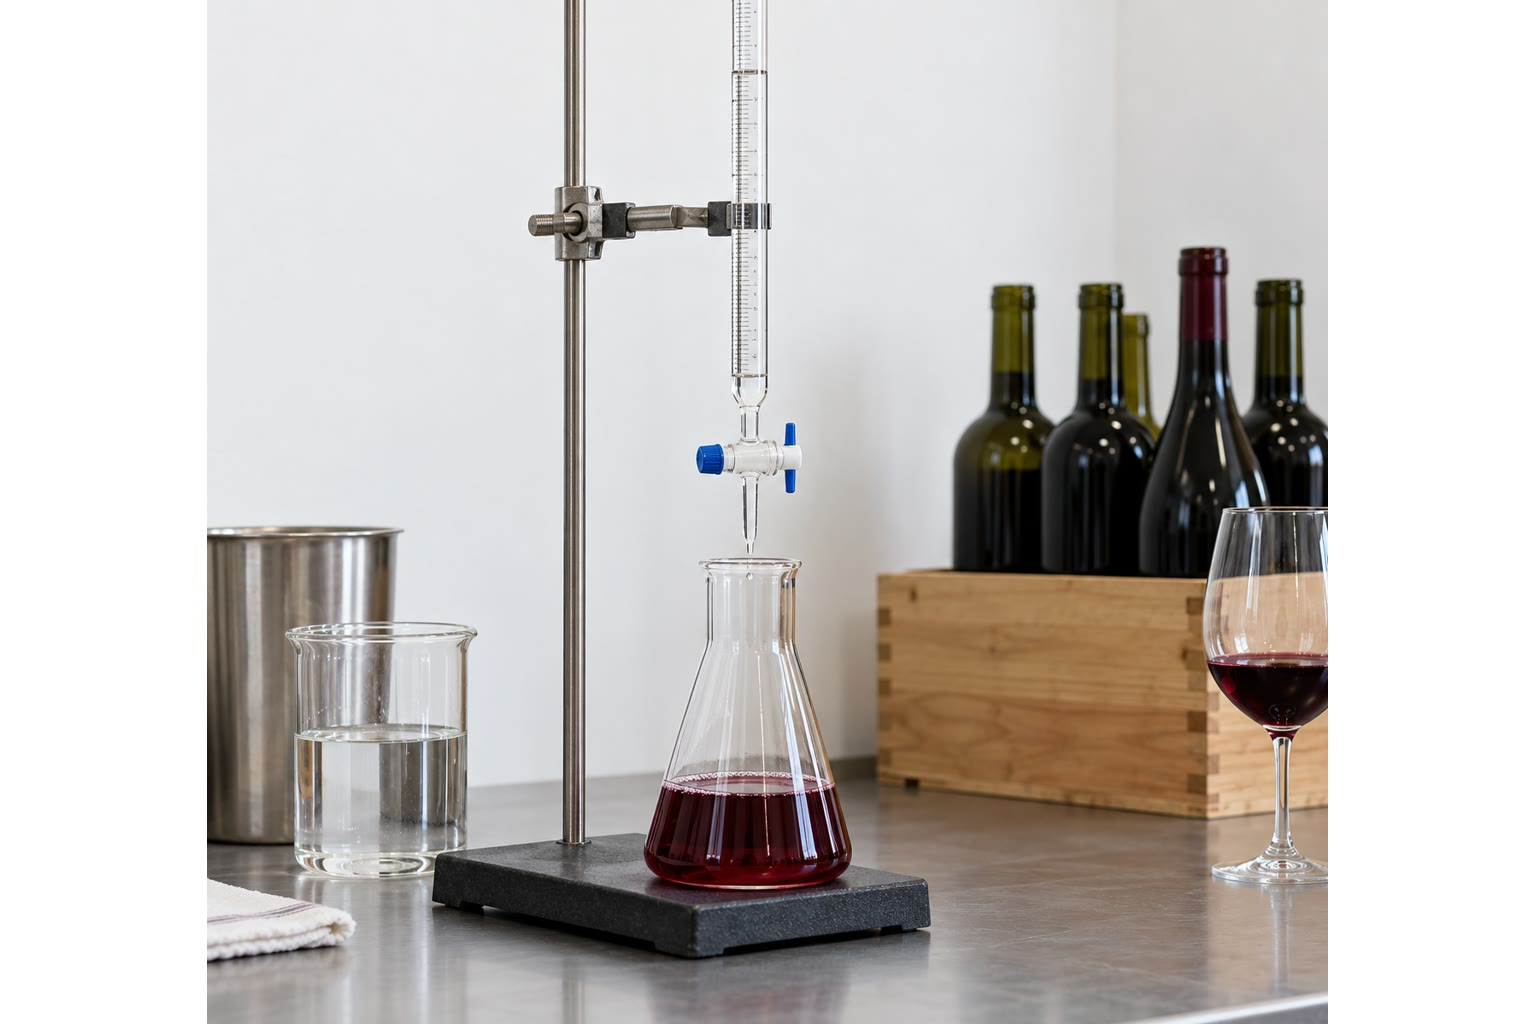
\includegraphics[width=0.45\linewidth]{images/book1/ai/g12-wine-lab.jpg}

{\small La paillasse de \omterm{def:g11:titration:titration}{titrage} d'un viticulteur.}
\end{omfigure}

\section{Le titrage pH-métrique}

\begin{definition}[Titrage pH-métrique, demi-équivalence]\label{def:g12:ph-conductivity-titrations:ph-metric}
Lors d'un \emph{titrage pH-métrique}\index{titrage ph-metrique@titrage pH-métrique}, on
mesure le \omterm{def:g9:acids-bases-ph:ph}{pH} de la \omterm{def:g11:titration:titration}{solution titrée} après chaque ajout de \omterm{def:g11:titration:titration}{solution
titrante}, et on trace la courbe du \omterm{def:g9:acids-bases-ph:ph}{pH} en fonction du volume versé. La
\emph{demi-équivalence}\index{demi-equivalence@demi-équivalence}
est le point où la moitié du \omterm{def:g11:titration:equivalence}{volume à l'équivalence} a été versée.
\end{definition}

\begin{omfigure}
\begin{tikzpicture}[font=\small, scale=0.65]
  \pic[transform shape] at (0,0) {stand={6.3}{2.0}};
  \pic[transform shape] at (2.0,0.68) {stirrer};
  \pic[transform shape] at (2.0,0.68) {beaker={0.45}{omWater}};
  \pic[transform shape] at (2.0,2.9) {burette={0.8}{omWater}};
  \pic[transform shape] (pr) at (2.6,0.95) {probe};
  \pic[transform shape] (m) at (6.4,3.4) {meter={pH}};
  \draw[black!70, thick] (pr-top) .. controls +(0,1.0) and +(0,-1.2) .. (m-a);
  \draw[omProp, thick, <-] (2.35,7.2) -- (4.3,7.6) node[right, text=black] {burette~: NaOH};
  \draw[omProp, thick, <-] (1.4,1.1) -- (-1.4,1.6) node[left, text=black, align=right] {acide à titrer};
  \draw[omProp, thick, <-] (2.75,2.4) -- (4.3,2.0) node[right, text=black] {sonde de pH};
\end{tikzpicture}

{\small Un \omterm{def:g12:ph-conductivity-titrations:ph-metric}{titrage pH-métrique}~: la sonde plonge dans la solution agitée,
l'appareil affiche le \omterm{def:g9:acids-bases-ph:ph}{pH} après chaque ajout.}
\end{omfigure}

\begin{inthelab}[Étalonner un pH-mètre]
Avant usage, on rince la sonde à l'eau distillée et on la plonge dans
deux \omterm{def:g12:buffers-predominance:buffer}{solutions tampons} de \omterm{def:g9:acids-bases-ph:ph}{pH} connu, en général 7.0 et 4.0 (ou 10.0)~:
on règle l'appareil pour qu'il affiche leurs valeurs. Entre deux
solutions, on rince la sonde et on la sèche délicatement en la
tamponnant, sans jamais l'essuyer~; on la conserve avec son extrémité
humide.
\end{inthelab}

\begin{omfigure}
\begin{minipage}{0.49\linewidth}
\begin{tikzpicture}
\begin{axis}[width=\linewidth, height=6cm, xmin=0, xmax=30, ymin=0, ymax=14,
    xlabel={$V_{\text{NaOH}}$ (\si{mL})}, ylabel={pH}, axis lines*=left,
    ymajorgrids, grid style={gray!20}, tick label style={font=\scriptsize},
    label style={font=\small}, title={\small \ce{HCl} par \ce{NaOH}},
    title style={yshift=-4pt}]
  \addplot[very thick, omDef] table[x=V, y=pH] {figdata/out/grade-12-ph-conductivity-titrations-a.dat};
  \addplot[thick, omProp, densely dotted] table[x=V, y expr=\thisrow{dpH}/4]
    {figdata/out/grade-12-ph-conductivity-titrations-a.dat};
  \addplot[dashed, black!60] coordinates {(20,0) (20,7)};
  \node[font=\scriptsize, anchor=north west] at (axis cs:20.3,6.5) {$V_E = 20.0$};
\end{axis}
\end{tikzpicture}
\end{minipage}\hfill
\begin{minipage}{0.49\linewidth}
\begin{tikzpicture}
\begin{axis}[width=\linewidth, height=6cm, xmin=0, xmax=16, ymin=0, ymax=14,
    xlabel={$V_{\text{NaOH}}$ (\si{mL})}, ylabel={pH}, axis lines*=left,
    ymajorgrids, grid style={gray!20}, tick label style={font=\scriptsize},
    label style={font=\small}, title={\small \ce{CH3COOH} par \ce{NaOH}},
    title style={yshift=-4pt}]
  \addplot[very thick, omDef] table[x=V, y=pH] {figdata/out/grade-12-ph-conductivity-titrations-b.dat};
  \addplot[thick, omProp, densely dotted] table[x=V, y expr=\thisrow{dpH}/4]
    {figdata/out/grade-12-ph-conductivity-titrations-b.dat};
  \addplot[dashed, black!60] coordinates {(10.1,0) (10.1,8.7)};
  \addplot[dashed, black!60] coordinates {(0,4.76) (5.05,4.76) (5.05,0)};
  \node[font=\scriptsize, anchor=south west] at (axis cs:0.2,4.8) {$pK_a = 4.76$};
  \node[font=\scriptsize, anchor=north west] at (axis cs:10.4,3.0) {$V_E = 10.1$};
\end{axis}
\end{tikzpicture}
\end{minipage}

{\small Courbes de \omterm{def:g9:acids-bases-ph:ph}{pH} calculées (en bleu) et leur dérivée
$d\mathrm{pH}/dV$
(en orange, en pointillés, divisée par 4). À gauche~: \qty{20.0}{mL}
d'acide chlorhydrique à \qty{0.100}{mol/L}~; \omterm{def:g11:titration:equivalence}{équivalence} à \omterm{def:g9:acids-bases-ph:ph}{pH} 7.00. À
droite~: \qty{10.0}{mL} de vinaigre dilué~; à la \omterm{def:g12:ph-conductivity-titrations:ph-metric}{demi-équivalence}, le
\omterm{def:g9:acids-bases-ph:ph}{pH} est égal au $pK_a$, et l'\omterm{def:g11:titration:equivalence}{équivalence} se situe à un \omterm{def:g9:acids-bases-ph:ph}{pH} basique.}
\end{omfigure}


\begin{method}[La méthode de la dérivée]\label{met:g12:ph-conductivity-titrations:derivative}
Calculer, entre deux mesures successives, la pente
$\Delta\mathrm{pH}/\Delta V$, et la représenter en fonction de $V$ (un
tableur ou une calculatrice s'en charge). Le \omterm{def:g11:titration:equivalence}{volume à l'équivalence}
correspond à la plus grande pente~: le pic de la courbe dérivée.
\end{method}

\begin{method}[La méthode des tangentes]\label{met:g12:ph-conductivity-titrations:tangent}
\begin{enumerate}
  \item Tracer deux tangentes parallèles à la courbe, l'une avant et
        l'autre après le saut, de part et d'autre de celui-ci.
  \item Tracer la parallèle située à égale distance des deux.
  \item Son intersection avec la courbe est le point d'\omterm{def:g11:titration:equivalence}{équivalence}~: on
        y lit $V_E$ (et le \omterm{def:g9:acids-bases-ph:ph}{pH} à l'\omterm{def:g11:titration:equivalence}{équivalence}).
\end{enumerate}
\end{method}

\begin{proposition}[À la demi-équivalence, $\mathrm{pH} = pK_a$]\label{prop:g12:ph-conductivity-titrations:half}
Lors du \omterm{def:g11:titration:titration}{titrage} d'un \omterm{def:g12:ka-and-pka:strong-acid}{acide faible} \ce{HA} par une \omterm{def:g12:ka-and-pka:strong-acid}{base forte}, à la
\omterm{def:g12:ph-conductivity-titrations:ph-metric}{demi-équivalence}, $\mathrm{pH} = pK_a$.
\end{proposition}

\begin{proof}
La réaction \ce{HA + OH- -> A- + H2O} est totale. À la \omterm{def:g12:ph-conductivity-titrations:ph-metric}{demi-équivalence},
la moitié
de l'acide a été transformée en \ce{A-}~: $[\ce{A-}] = [\ce{HA}]$, et
la relation de Henderson donne $\mathrm{pH} = pK_a + \log 1 = pK_a$.
\end{proof}

\begin{remark}[Choisir un indicateur à partir de la courbe]\label{rem:g12:ph-conductivity-titrations:indicator}
% ledger: ind:BBT, ind:phenolphthalein
L'indicateur doit changer de couleur à l'intérieur du saut. Pour l'acide
chlorhydrique, le saut s'étend environ de \omterm{def:g9:acids-bases-ph:ph}{pH} 4 à 10 et de nombreux
indicateurs conviennent, le bleu de bromothymol au mieux~; pour l'acide
éthanoïque, le saut est plus court et basique, environ de 7 à 11~: la
phénolphtaléine (8.0--10.0) convient, le bleu de bromothymol virerait
trop tôt.
\end{remark}

\section{Conductivité et titrages conductimétriques}

\begin{definition}[Conductivité, conductivité molaire ionique]\label{def:g12:ph-conductivity-titrations:conductivity}
La \emph{conductivité}\index{conductivite@conductivité} $\sigma$ d'une solution
mesure son aptitude à conduire le courant électrique~; on la lit sur un
conductimètre, en \si{mS/cm} (ou en \si{S/m}). Chaque \omterm{def:g9:ions:ion}{ion} $i$ y
contribue proportionnellement à sa concentration, avec un coefficient
$\lambda_i$, sa
\emph{conductivité molaire ionique}\index{conductivite molaire ionique@conductivité molaire ionique}.
\end{definition}

\begin{proposition}[Loi de Kohlrausch]\label{prop:g12:ph-conductivity-titrations:kohlrausch}
% ledger: lam:H+, lam:OH-, lam:Na+, lam:Cl-
Pour une solution diluée, $\sigma = \sum_i \lambda_i [X_i]$. À
\qty{25}{\celsius}, en \si{S.cm^2/mol}~: \ce{H3O+} 349.8, \ce{OH-}
198.3,
\ce{Cl-} 76.2, \ce{Na+} 50.3. Les \omterm{def:g12:ka-and-pka:oxonium}{ions oxonium} et hydroxyde conduisent
bien mieux que tous les autres \omterm{def:g9:ions:ion}{ions}.
\end{proposition}

\begin{proof}
Admis (volume de première année d'université). Les valeurs de \ce{Cl-}
et de \ce{Na+} proviennent
des \omterm{def:g12:ph-conductivity-titrations:conductivity}{conductivités} mesurées de solutions d'acide chlorhydrique et de
chlorure de sodium, dont on retranche celle de \ce{H3O+}.
\end{proof}

\begin{definition}[Titrage conductimétrique]\label{def:g12:ph-conductivity-titrations:conductimetric}
Lors d'un \emph{titrage conductimétrique}\index{titrage conductimetrique@titrage conductimétrique},
on mesure la \omterm{def:g12:ph-conductivity-titrations:conductivity}{conductivité} après chaque ajout de \omterm{def:g11:titration:titration}{solution titrante}. La
\omterm{def:g11:titration:titration}{solution titrée} est diluée dans un grand volume d'eau, de sorte que le
volume ajouté la modifie à peine~: les points sont alors alignés sur des
droites, qui changent de pente à l'\omterm{def:g11:titration:equivalence}{équivalence}.
\end{definition}

\begin{omfigure}
\begin{minipage}{0.4\linewidth}\centering
\begin{tikzpicture}[font=\small, scale=0.75]
  \pic[transform shape] at (0,0) {beaker={0.6}{omWater}};
  \pic[transform shape] (cc) at (0.2,0.2) {condcell};
  \pic[transform shape] (m) at (2.6,3.4) {meter={mS/cm}};
  \draw[black!70, thick] (cc-top) .. controls +(0,0.8) and +(0,-1) .. (m-a);
  \node[anchor=north, align=center] at (0.6,-0.15) {cellule de conductimétrie\\ dans la solution};
\end{tikzpicture}
\end{minipage}\hfill
\begin{minipage}{0.56\linewidth}
\begin{tikzpicture}
\begin{axis}[width=\linewidth, height=5.4cm, xmin=0, xmax=20, ymin=0,
    ymax=4.6, xlabel={$V_{\text{NaOH}}$ (\si{mL})}, ylabel={$\sigma$ (\si{mS/cm})},
    axis lines*=left, ymajorgrids, grid style={gray!20},
    tick label style={font=\scriptsize}, label style={font=\small}]
  \addplot[only marks, mark=*, mark size=1.4pt, omDef] table[x=V, y=sigma]
    {figdata/out/grade-12-ph-conductivity-titrations-c.dat};
  \addplot[dashed, black!60] coordinates {(10,0) (10,4.6)};
  \node[font=\scriptsize, anchor=south west] at (axis cs:10.3,0.2) {$V_E = 10.0$};
\end{axis}
\end{tikzpicture}
\end{minipage}

{\small À gauche~: une cellule de conductimétrie. À droite~:
\qty{100}{mL} d'acide chlorhydrique à \qty{0.0100}{mol/L} titrés par de
l'hydroxyde de sodium à
\qty{0.100}{mol/L} (valeurs calculées avec la loi de Kohlrausch). La
\omterm{def:g12:ph-conductivity-titrations:conductivity}{conductivité} diminue, puis augmente~: deux droites qui se coupent à
l'\omterm{def:g11:titration:equivalence}{équivalence}.}
\end{omfigure}

\begin{example}[Lire les deux droites]\label{ex:g12:ph-conductivity-titrations:lines}
Avant l'\omterm{def:g11:titration:equivalence}{équivalence}, chaque \omterm{def:g9:ions:ion}{ion} \ce{OH-} ajouté fait disparaître un \omterm{def:g9:ions:ion}{ion}
\ce{H3O+}
($\lambda = 349.8$) et apporte un \omterm{def:g9:ions:ion}{ion} \ce{Na+} ($\lambda = 50.3$)~: la
\omterm{def:g12:ph-conductivity-titrations:conductivity}{conductivité} diminue fortement. Après l'\omterm{def:g11:titration:equivalence}{équivalence}, les \omterm{def:g9:ions:ion}{ions} \ce{Na+}
et \ce{OH-}
($\lambda = 198.3$) s'accumulent simplement~: elle augmente. Les deux
droites se coupent en
$V_E = \qty{10.0}{mL}$, donc la concentration de l'acide était
$0.100 \times 10.0 / 100 = \qty{0.0100}{mol/L}$.
\end{example}

\begin{method}[L'équivalence d'un titrage conductimétrique]\label{met:g12:ph-conductivity-titrations:two-lines}
Tracer la droite qui passe au mieux par les points situés avant
l'\omterm{def:g11:titration:equivalence}{équivalence} et celle qui passe au mieux par les points situés après~;
lire $V_E$ à leur intersection. On écarte les points proches de
l'\omterm{def:g11:titration:equivalence}{équivalence}, là où les droites s'incurvent.
\end{method}

\begin{remark}[Quelle méthode, et quand]\label{rem:g12:ph-conductivity-titrations:which}
Un indicateur coloré est le plus rapide quand il en existe un qui
convient. Un \omterm{def:g12:ph-conductivity-titrations:ph-metric}{titrage pH-métrique} donne en plus le $pK_a$ d'un \omterm{def:g12:ka-and-pka:strong-acid}{acide
faible}, et fonctionne avec des solutions colorées ou troubles. Un
\omterm{def:g12:ph-conductivity-titrations:conductimetric}{titrage conductimétrique} n'a besoin d'aucun saut de \omterm{def:g9:acids-bases-ph:ph}{pH}~: il convient
aux acides très faibles ou très dilués, et aux réactions de
\omterm{def:g9:ions:precipitate}{précipitation}, du moment que les \omterm{def:g9:ions:ion}{ions} changent.
\end{remark}

\begin{safety}{\ghs[0.82cm]{GHS05}\ghs[0.82cm]{GHS07}}
% ledger: ghs:NaOH
Les solutions d'hydroxyde de sodium brûlent la peau et les yeux, même
diluées pour les yeux~: lunettes en permanence, et toute projection est
rincée aussitôt à grande eau.
\end{safety}

\section{Exercices}


\begin{exercise}[$\star$]\label{exo:g12:ph-conductivity-titrations:1}
Lire le \omterm{def:g11:titration:equivalence}{volume à l'équivalence} sur la courbe de l'acide chlorhydrique
titré par l'hydroxyde de sodium à \qty{0.100}{mol/L}, et en déduire la
concentration des \qty{20.0}{mL} d'acide.
\end{exercise}

\begin{exercise}[$\star$]\label{exo:g12:ph-conductivity-titrations:2}
On titre un \omterm{def:g12:ka-and-pka:strong-acid}{acide faible} par l'hydroxyde de sodium~; $V_E = \qty{12.0}{mL}$.
À
\qty{6.0}{mL}, le \omterm{def:g9:acids-bases-ph:ph}{pH} vaut 3.75. Donner le $pK_a$ de l'acide. De quel
acide de l'échelle des $pK_a$ pourrait-il s'agir~?
\end{exercise}

\begin{exercise}[$\star$]\label{exo:g12:ph-conductivity-titrations:3}
Quel indicateur choisir pour le \omterm{def:g11:titration:titration}{titrage} de l'acide éthanoïque par
l'hydroxyde de sodium~? Pourquoi pas le rouge de méthyle~?
\end{exercise}

\begin{exercise}[$\star$]\label{exo:g12:ph-conductivity-titrations:4}
Pourquoi faut-il étalonner un \omterm{def:g9:acids-bases-ph:ph-paper}{pH-mètre} avant usage~? Avec quoi~?
\end{exercise}

\begin{exercise}[$\star$]\label{exo:g12:ph-conductivity-titrations:5}
À l'aide des \omterm{def:g12:ph-conductivity-titrations:conductivity}{conductivités molaires ioniques}, classer les \omterm{def:g9:ions:ion}{ions}
\ce{H3O+}, \ce{OH-},
\ce{Na+}, \ce{Cl-} du meilleur conducteur au moins bon.
\end{exercise}

\begin{exercise}[$\star\star$]\label{exo:g12:ph-conductivity-titrations:6}
\qty{20.0}{mL} d'une solution d'acide éthanoïque demandent
\qty{14.6}{mL} d'hydroxyde de sodium à \qty{0.050}{mol/L}. Calculer sa
concentration.
\end{exercise}

\begin{exercise}[$\star\star$]\label{exo:g12:ph-conductivity-titrations:7}
Près de l'\omterm{def:g11:titration:equivalence}{équivalence}, on relève~: \qty{9.6}{mL}, \omterm{def:g9:acids-bases-ph:ph}{pH} 5.7~;
\qty{9.8}{mL}, 6.1~; \qty{10.0}{mL}, 7.0~; \qty{10.2}{mL}, 10.5~;
\qty{10.4}{mL}, 11.0. Calculer $\Delta\mathrm{pH}/\Delta V$ entre deux
points successifs et repérer $V_E$.
\end{exercise}

\begin{exercise}[$\star\star$]\label{exo:g12:ph-conductivity-titrations:8}
Lors du \omterm{def:g12:ph-conductivity-titrations:conductimetric}{titrage conductimétrique} de l'acide chlorhydrique, expliquer le
signe de la pente avant et après l'\omterm{def:g11:titration:equivalence}{équivalence}, à l'aide des \omterm{def:g9:ions:ion}{ions}
présents.
\end{exercise}

\begin{exercise}[$\star\star$]\label{exo:g12:ph-conductivity-titrations:9}
Esquisser la courbe de \omterm{def:g12:ph-conductivity-titrations:conductimetric}{titrage conductimétrique} de l'acide éthanoïque
par l'hydroxyde de sodium. Pourquoi la \omterm{def:g12:ph-conductivity-titrations:conductivity}{conductivité} augmente-t-elle dès
avant l'\omterm{def:g11:titration:equivalence}{équivalence}~?
\end{exercise}

\begin{exercise}[$\star\star$]\label{exo:g12:ph-conductivity-titrations:10}
Sur la courbe calculée du vinaigre dilué, lire le \omterm{def:g9:acids-bases-ph:ph}{pH} au départ, à la
\omterm{def:g12:ph-conductivity-titrations:ph-metric}{demi-équivalence} et à l'\omterm{def:g11:titration:equivalence}{équivalence}. Pourquoi le \omterm{def:g9:acids-bases-ph:ph}{pH} de départ est-il
bien plus élevé que celui de l'acide chlorhydrique à la même
concentration~?
\end{exercise}

\begin{exercise}[$\star\star$]\label{exo:g12:ph-conductivity-titrations:11}
Pourquoi dilue-t-on la \omterm{def:g11:titration:titration}{solution titrée} dans un grand volume d'eau avant
un \omterm{def:g12:ph-conductivity-titrations:conductimetric}{titrage conductimétrique}~?
\end{exercise}

\begin{exercise}[$\star\star\star$]\label{exo:g12:ph-conductivity-titrations:12}
Une solution contient à la fois de l'acide chlorhydrique et de l'acide
éthanoïque. On la titre par l'hydroxyde de sodium en mesurant le \omterm{def:g9:acids-bases-ph:ph}{pH}.
Expliquer pourquoi la courbe présente deux sauts, et ce que mesure
chaque \omterm{def:g11:titration:equivalence}{volume à l'équivalence}.
\end{exercise}

\begin{exercise}[$\star\star\star$]\label{exo:g12:ph-conductivity-titrations:13}
Calculer la \omterm{def:g12:ph-conductivity-titrations:conductivity}{conductivité} au début du \omterm{def:g12:ph-conductivity-titrations:conductimetric}{titrage conductimétrique} du
chapitre (acide chlorhydrique à \qty{0.0100}{mol/L}) et à l'\omterm{def:g11:titration:equivalence}{équivalence}
(\qty{110}{mL} de solution de chlorure de sodium). Comparer avec la
figure.
\end{exercise}

\begin{exercise}[$\star\star\star$]\label{exo:g12:ph-conductivity-titrations:14}
Un \omterm{def:g9:acids-bases-ph:ph-paper}{pH-mètre} mal étalonné indique tous les \omterm{def:g9:acids-bases-ph:ph}{pH} avec 0.2 unité de trop.
Quelle erreur cela entraîne-t-il sur le \omterm{def:g11:titration:equivalence}{volume à l'équivalence} d'un
\omterm{def:g12:ph-conductivity-titrations:ph-metric}{titrage pH-métrique}~? Sur le $pK_a$
lu à la \omterm{def:g12:ph-conductivity-titrations:ph-metric}{demi-équivalence}~?
\end{exercise}

\begin{exercise}[$\star\star\star$]\label{exo:g12:ph-conductivity-titrations:15}
Pourquoi un \omterm{def:g12:ph-conductivity-titrations:conductimetric}{titrage conductimétrique} peut-il suivre la réaction des \omterm{def:g9:ions:ion}{ions}
argent avec les \omterm{def:g9:ions:ion}{ions} chlorure, \ce{Ag+ + Cl- -> AgCl(s)}, alors qu'un
\omterm{def:g12:ph-conductivity-titrations:ph-metric}{titrage pH-métrique} ne le peut pas~? Décrire la courbe attendue quand on
ajoute du nitrate d'argent à du chlorure de sodium (prendre pour
$\lambda$ de \ce{NO3-} une valeur voisine de celle de
\ce{Cl-}).
\end{exercise}

\section{Problème~: le vinaigre est-il à 6\,\%~?}

\begin{problem}[{Problème du week-end --- un vinaigre étiqueté «~6~\%
d'acidité~» contient-il vraiment six grammes d'acide éthanoïque pour
cent grammes~?}]
\label{pb:g12:ph-conductivity-titrations:1}
% ledger: pka:ethanoic, ind:phenolphthalein, lam:OH-, lam:Na+, aw:C, aw:H, aw:O
On contrôle un vinaigre étiqueté «~6~\% d'acidité~». On en pèse
\qty{100.0}{mL}~: \qty{101}{g}. On dilue le vinaigre dix fois, puis on
titre \qty{10.0}{mL} de la solution diluée par de l'hydroxyde de sodium
à \qty{0.100}{mol/L}, en suivant le \omterm{def:g9:acids-bases-ph:ph}{pH}~; la courbe calculée du
chapitre (à droite) correspond aux mesures.

\medskip
\noindent\textbf{Partie I --- Préparer l'échantillon.}
\begin{enumerate}
  \item Que signifie «~6~\% d'acidité~»~?
  \item Si l'étiquette dit vrai, quelle masse d'acide éthanoïque
        \qty{100.0}{mL} de vinaigre contiennent-ils~? À quelle
        \omterm{def:g10:concentration-and-dilution:molar-concentration}{concentration molaire} cela correspond-il~?
  \item Pourquoi dilue-t-on le vinaigre avant le \omterm{def:g11:titration:titration}{titrage}~?
  \item Quelle verrerie utilise-t-on pour le diluer dix fois~?
\end{enumerate}

\medskip
\noindent\textbf{Partie II --- Le \omterm{def:g12:ph-conductivity-titrations:ph-metric}{titrage pH-métrique}.}
\begin{enumerate}[resume]
  \item Écrire l'équation de la réaction de \omterm{def:g11:titration:titration}{titrage}.
  \item Lire le \omterm{def:g11:titration:equivalence}{volume à l'équivalence} sur la courbe.
  \item Calculer la concentration du vinaigre dilué.
  \item En déduire celle du vinaigre.
  \item Lire le \omterm{def:g9:acids-bases-ph:ph}{pH} à la \omterm{def:g12:ph-conductivity-titrations:ph-metric}{demi-équivalence}. Que donne-t-il~?
  \item Pourquoi le \omterm{def:g9:acids-bases-ph:ph}{pH} à l'\omterm{def:g11:titration:equivalence}{équivalence} est-il supérieur à 7~?
  \item Quel indicateur aurait donné le même résultat~?
\end{enumerate}

\medskip
\noindent\textbf{Partie III --- Une vérification conductimétrique.}
\begin{enumerate}[resume]
  \item On recommence le \omterm{def:g11:titration:titration}{titrage} avec une cellule de conductimétrie,
        l'échantillon étant dilué dans \qty{200}{mL} d'eau. Quels \omterm{def:g9:ions:ion}{ions}
        apparaissent dans la solution avant l'\omterm{def:g11:titration:equivalence}{équivalence}~?
  \item Pourquoi la \omterm{def:g12:ph-conductivity-titrations:conductivity}{conductivité} n'augmente-t-elle que lentement avant
        l'\omterm{def:g11:titration:equivalence}{équivalence}~?
  \item Pourquoi augmente-t-elle plus vite après~?
  \item Pourquoi la \omterm{def:g12:ph-conductivity-titrations:conductivity}{conductivité} est-elle très faible au départ~?
  \item Où les deux droites doivent-elles se couper~?
\end{enumerate}

\medskip
\noindent\textbf{Partie IV --- Le verdict.}
\begin{enumerate}[resume]
  \item Calculer la \omterm{def:g10:concentration-and-dilution:mass-concentration}{concentration massique} en acide éthanoïque du
        vinaigre.
  \item Calculer la masse d'acide éthanoïque dans \qty{100.0}{mL} de
        vinaigre.
  \item En déduire la masse d'acide éthanoïque pour \qty{100}{g} de
        vinaigre.
  \item Donner la réponse finale~: quelle est l'acidité du vinaigre~?
\end{enumerate}
\end{problem}
